\subsection{Decision 5: Database scope and organization}

\subsection*{Status}
Accepted. Reviewed after Decision 10 (Data update from Tycoons). Reviewed after Decision 8 (Scanner interactions) to add a User State database.

\subsection*{Architectural Summary}
\begin{tabular}{|p{3.5cm}|p{10.5cm}|}
    \hline
    \textbf{In the context of} & Choosing which data should be stored in the TrIP system, \\
    \hline
    \textbf{Facing} & The challenge of ensuring data security and high performance, \\
    \hline
    \textbf{To achieve} & High performance in data retrieval, easy integrability with tycoons' systems, \\
    \hline
    \textbf{We considered} & Option 1: Database-per-service pattern; Option 2: Unified Centralized Database System; Option 3: Database per tycoon, Option 4: Hybrid cloud storage\\
    \hline
    \textbf{And decided for} & Option 1: Database-per-service pattern, Option 4: Hybrid cloud storage \\
    \hline
    \textbf{Because} & It allows us to achieve high availabiliy and maintenability, \\
    \hline
    \textbf{Accepting} & Increased System Complexity, higher costs. \\
    \hline
\end{tabular}

\subsection*{Context}
We need to answer the following questions:
\begin{itemize}
\item Which info do we keep in the database? 
\item Do we need one or many databases?
\item How do we handle data protection?
\item How do we handle data update from tycoons/station management? (maybe for another decision?)
\end{itemize}

\subsection*{Concern}
We need to keep some information available from our system, but security of the data (especially payment and account data) is crucial for the government and for the passengers concerns.
We also need high performance in giving routes choices to passengers and quick payments.

The following user stories are particularly relevant to the decision on the database scope, emphasizing the need for comprehensive management of subscriptions, security, and system integration:

\begin{itemize}[noitemsep]
    \item \userStoryOne, 
    \item \userStoryTwo,
    \item \userStoryFour,
    \item \userStorySixteen,
    \item \userStoryEighteen,
    \item \userStoryTwentyThree,
    \item \userStoryTwentySeven,
\end{itemize}

\subsection*{Criteria}
\begin{itemize}[noitemsep]
    \item \textit{Performance and availability}: Quick and reliable data retrieval.
    \item \textit{Mainteinability}: clear data organization and division of responsibilities across system elements.
    \item \textit{Security}: Protection of sensitive data.
\end{itemize}

\subsection*{Option 1: Database-per-service pattern}
We try to have one database for each important set of information that the system needs to know, employing the database-per-service pattern.
We try to stick to the Separation of Concerns principle, so that each module only has access to the data it scricly needs to operate.
We divide the following:
\begin{itemize}
    \item A database containing the timetable, the prices of seats and the bookings.
    \item A database containing the optimized routes cached after being calculated by the Routes Optimization Module.
    \item A database containing info about the accounts and their subscriptions. 
    \item A database recording payments that have been done, which should be accessed in case for example of complaints. 
\end{itemize}
\begin{figure}[ht]
    \centering
    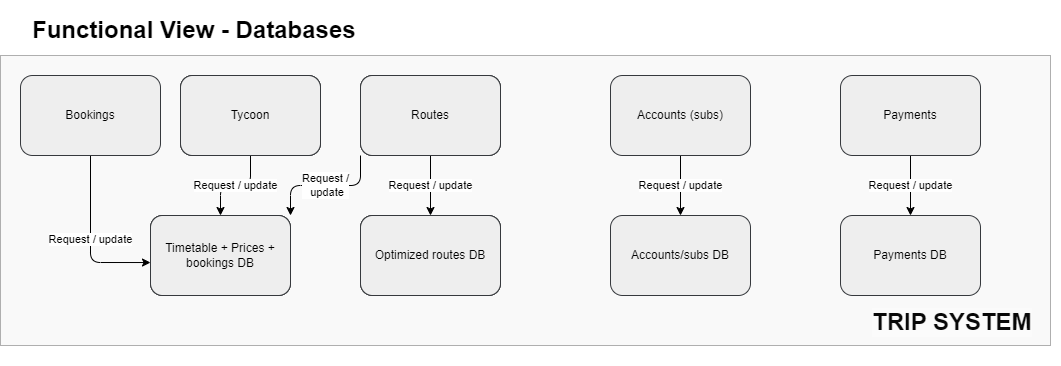
\includegraphics[width=\textwidth]{drawings/views_draft2/functional_view databases.png}
    \caption{Division of databases and their interaction with modules or stakeholders.}
    \label{fig:databases_view}
\end{figure}

\subsubsection*{Pros}
\begin{itemize}[noitemsep]
    \item \textbf{Enhanced Security} (Data Protection, Privacy): By segregating data across multiple databases, sensitive information is better protected, and access can be tightly controlled on a need-to-know basis.
    \item \textbf{Specialized Optimization} (Performance, Efficiency): Dedicated databases allow for optimization specific to their function, such as faster queries for timetable and booking data versus complex route optimization calculations.
\end{itemize}

\subsubsection*{Cons}
\begin{itemize}[noitemsep]
    \item \textbf{Increased Maintenance Overhead} (Maintainability, Complexity): Managing multiple databases adds complexity to the system's architecture, requiring more resources for maintenance and potentially higher costs.
    \item \textbf{Data Synchronization Challenges} (Reliability, Consistency): Ensuring data consistency across different databases can be challenging, especially in real-time, and may affect the system's overall reliability.
\end{itemize}

\subsection*{Option 2: Unified Centralized Database System}

This option proposes a centralized database architecture that consolidates all necessary information into a single, unified database system. It incorporates robust access control layers to manage data access based on module or user roles, ensuring that each part of the system accesses only the data it needs for operation. This model simplifies data management, enhances security through centralized control mechanisms, and facilitates easier updates and integrations. This model can be improved with having accounts database as a separate component, and keeping the rest of the databases central. In this way accounts data will be secure, and the rest of the systems will access accounts data anonymously via ids. Manage permissions for eacsh tycoon, on which info they can access (they shouldn't be able to connect name to bank account). In this way we can keep everything in the same place, but each tycoon api will have specificed access protocols. Tycoons can only update timetables and prices.

We can keep bookings data a DaaS, since it needs to be updated regularly and concurrently. The rest can be a server based database. Since we can cache routes we don't want cloud services for these. 

\subsubsection*{Pros}
\begin{itemize}[noitemsep]
    \item \textbf{Simplified Data Management} (Maintainability, Efficiency): Centralizing data storage simplifies the architecture by reducing the number of systems to manage, making it easier to maintain and update the database.
    \item \textbf{Improved Data Consistency} (Reliability, Integrity): A unified database ensures that all modules access the most current and consistent data, reducing the risk of discrepancies and errors.
    \item \textbf{Enhanced Integration Capability} (Scalability, Interoperability): With all data in one place, integrating new features, modules, or external systems becomes more straightforward, promoting scalability and interoperability.
\end{itemize}

\subsubsection*{Cons}
\begin{itemize}[noitemsep]
    \item \textbf{Risk of a Single Point of Failure} (Reliability, Availability): Centralizing data creates a single point of failure, which could potentially lead to system-wide outages affecting all functionalities if the database goes down.
    \item \textbf{Scalability Concerns} (Performance, Scalability): As the system grows, a centralized database might struggle with performance issues due to the increasing volume of data and concurrent access requests.
    \item \textbf{Complexity in Ensuring Data Protection} (Security, Privacy): Protecting a large, centralized repository of sensitive information poses significant challenges, requiring robust security measures to prevent unauthorized access and data breaches.
\end{itemize}

\subsection*{Option 3: Database per tycoon}

This option involves creating separate databases for each tycoon, allowing tailored data management and access controls specific to the needs and permissions of each tycoon. The aim is to provide a customized data storage solution that respects the autonomy and specific requirements of each railway tycoon, facilitating efficient and secure data handling.

\subsubsection*{Pros}
\begin{itemize}
    \item \textbf{Customization:} Each tycoon can have database features and structures tailored to their specific operational and data analysis needs, enhancing performance and usability.
    \item \textbf{Access Control:} Tycoon-specific databases simplify permission management, as each tycoon has access only to their relevant database, thereby automatically managing access permissions and minimizing the risk of unauthorized data access.
\end{itemize}

\subsubsection*{Cons}
\begin{itemize}
    \item \textbf{Management Overhead:} Maintaining separate databases for each tycoon increases the complexity of the system's architecture, requiring more resources for database management, synchronization, and ensuring consistency across databases.
    \item \textbf{Data Redundancy:} Shared data that is relevant to multiple tycoons, such as inter-tycoon route connections or passenger information, may need to be duplicated across databases, increasing storage requirements and complicating data synchronization.
\end{itemize}

This option was considered to provide high levels of customization and security by isolating each tycoon's data. However, it introduces significant challenges in terms of system complexity and data management efficiency. The requirement for tailored solutions for each tycoon, while beneficial for customization and security, potentially complicates the integration and consistent operation of the TrIP system as a whole.


\subsection*{Option 4: Hybrid cloud storage}
Less sensitive data can be stored in public cloud (timetables, and prices and bookings). Sensitive data (accounts, payments) gets stored in non-cloud databases, possibly one per tycoon, to avoid illegal data access.

\subsubsection*{Pros}
\begin{itemize}[noitemsep]
    \item \textbf{Tycoon specific access for accounts data} 
    \item \textbf{Secure and qucik access to data crucial data} 
    \item \textbf{Cheap storage for non-crucial data} 
\end{itemize}

\subsubsection*{Cons}
\begin{itemize}[noitemsep]
    \item \textbf{Can get expensive} 
    \item \textbf{Implementation of two different database types and their interactions setup}
\end{itemize}

\subsection*{Decision}

In adopting a hybrid cloud storage strategy (Option 4), we remain committed to the database-per-service pattern (Option 1), ensuring a modular and scalable system architecture. The majority of our data, including timetables, prices, and bookings, will be stored in public cloud services to benefit from their scalability and operational efficiency. Sensitive information, such as passenger and payment data, will be secured in private servers, maintaining strict adherence to security and compliance standards. This dual approach, combining the use of public cloud and private servers, aligns with our commitment to both security and efficiency. It also preserves the modularity and service-specific scalability afforded by the database-per-service pattern. Detailed deployment strategies and justifications are further elaborated in the deployment viewpoint documentation.
The goal is to achive high availability, which is crucial after Event 2, which requires less stringent maintainability and cost requirements. Maintainability and performance are increased by choosing database-per-service instead of a single database.

\subsection*{Consequences}

\textbf{Positive Consequences:}
\begin{itemize}
    \item Enhanced security for sensitive data by utilizing private servers, aligning with strict compliance and privacy standards.
    \item Improved scalability and operational efficiency for non-sensitive data through the use of public cloud services.
    \item Retained system modularity and ease of maintenance via the database-per-service pattern, facilitating targeted optimizations and updates.
\end{itemize}

\textbf{Negative Consequences:}
\begin{itemize}
    \item Potential complexity in managing a hybrid cloud environment, requiring robust synchronization and data management practices.
    \item Increased operational demands for ensuring seamless integration and security protocols between public cloud services and private servers.
\end{itemize}